% proposal.tex

% Build settings & preferences:
\documentclass[a4paper,oneside]{bth}
\usepackage{etoolbox} % Toggle Conditionals.
\newtoggle{releasebuild}
\toggletrue{releasebuild} % Enable for Release build.
%\togglefalse{releasebuild} % Enable for Editorial build.

% proposalterms.tex
% Defines commonly used text to avoid spending time on formatting later on (in case APIs are later decided to be rendered in italics, for example):

\usepackage[utf8]{inputenc} % Because of Swedish characters in names.

% Document & Grammar:
\newcommand{\termsec}{Section}
\newcommand{\termcha}{Chapter}
\newcommand{\termproposal}{Proposal}
\newcommand{\termthesis}{Thesis}
\newcommand{\termeg}{e.g.}
% General & Abbreviations:
\newcommand{\termos}{OS}
\newcommand{\termttm}{TTM} % Time-to-Market
\newcommand{\termsdk}{SDK} % Software Development Kit
\newcommand{\termapi}{API} % Application Programming Interface
\newcommand{\termabi}{ABI} % Application Binary Interface
\newcommand{\termcpu}{CPU} % Central Processing Unit
\newcommand{\termgpu}{GPU} % Graphics Processing Unit
\newcommand{\termgpgpu}{GPGPU} % General Purpose computing on Graphics Processing Units
\newcommand{\termcallback}{Callback}
\newcommand{\termcompsci}{Computer~Science}
\newcommand{\termmips}{MIPS}
\newcommand{\termisa}{ISA}
\newcommand{\termfps}{FPS}
\newcommand{\termrw}{R/W}
% APIs & Technologies:
\newcommand{\termegl}{EGL}
\newcommand{\termxgl}{XGL}
\newcommand{\termagl}{AGL}
\newcommand{\termwgl}{WGL}
\newcommand{\termopengl}{OpenGL}
\newcommand{\termopengles}{\termopengl ~ES}
\newcommand{\termunix}{UNIX}
\newcommand{\termwinthirtytwo}{Win32}
\newcommand{\termip}{IP}
\newcommand{\termtcp}{TCP}
\newcommand{\termmac}{MAC}
\newcommand{\termarm}{ARM}
\newcommand{\termxeightysix}{x86}
% Organizations:
\newcommand{\termintel}{Intel~Corporation}
\newcommand{\termnvidia}{Nvidia}
\newcommand{\termgoogle}{Google}
\newcommand{\termwindriver}{Wind~River~Systems,~Inc.}
\newcommand{\termbth}{Blekinge~Institute~of~Technology}
\newcommand{\termbthdept}{Dept.~\termcompsci ~\&~Engineering}
\newcommand{\termmicrosoft}{Microsoft}
\newcommand{\termibm}{IBM}
\newcommand{\termacm}{ACM}
\newcommand{\termnasa}{NASA}
\newcommand{\termlinaro}{Linaro}
% Operating Systems, Technologies & Products:
\newcommand{\termosx}{OS~X}
\newcommand{\termlinux}{Linux}
\newcommand{\termsolaris}{Solaris}
\newcommand{\termandroid}{Android}
\newcommand{\termwindows}{\termmicrosoft ~Windows}
\newcommand{\termqemu}{QEMU}
\newcommand{\termandroidemu}{\termandroid ~Emulator}
\newcommand{\termvirgilthreed}{Virgil3D}
\newcommand{\termcuda}{CUDA}
\newcommand{\termdirectx}{Direct~X}
\newcommand{\termwarp}{WARP}
\newcommand{\termpci}{PCI}
\newcommand{\termxeleven}{X11}
\newcommand{\termglmarktwo}{glmark2}
% Simics:
\newcommand{\termsimics}{Simics}
\newcommand{\termfs}{\termsimics ~FS}
% Code-names:
\newcommand{\termrefimpl}{Reference~Implementation}
\newcommand{\termrefsolu}{Reference~Solution}
% Concepts:
\newcommand{\termtimetomarket}{\dvcmdcaponce{Time-to-Market}}
\newcommand{\termframespersecond}{\dvcmdcaponce{Frames Per Second}}
\newcommand{\termdetexe}{\dvcmdcaponce{Deterministic Execution}}
\newcommand{\termdetalg}{\dvcmdcaponce{Deterministic Algorithm}}
\newcommand{\termcheckpoint}{\dvcmdcaponce{Checkpoint}}
\newcommand{\termcheckpointrestart}{\dvcmdcaponce{Checkpoint / Restart}}
\newcommand{\termcheckpointing}{\dvcmdcaponce{Checkpointing}}
\newcommand{\termrevexe}{\dvcmdcaponce{Reverse Execution}}
\newcommand{\termtiming}{\dvcmdcaponce{Timing}}
\newcommand{\termhost}{\dvcmdcaponce{Host}}
\newcommand{\termtarget}{\dvcmdcaponce{Target}}
\newcommand{\termmagicinstr}{\dvcmdcaponce{Magic Instruction}}
\newcommand{\termparavirtualization}{\dvcmdcaponce{Paravirtualization}}
\newcommand{\termmillioninstructionspersecond}{\dvcmdcaponce{Million Instructions Per Second}}
% Persons involved in the project (in case titles are to be added):
\newcommand{\termhakan}{Prof. Håkan Grahn, Research Dean of Faculty}
\newcommand{\termhakandept}{Dept.~Computer~Science~\&~Engineering}
\newcommand{\termhakanemail}{\href{mailto:Hakan.Grahn@bth.se}{Hakan.Grahn@bth.se}}
\newcommand{\termdaniel}{Daniel~Aarno}
\newcommand{\termdanielemail}{\href{mailto:Daniel.Aarno@intel.com}{Daniel.Aarno@intel.com}}
\newcommand{\termdanieldept}{\termintel }
\newcommand{\termerik}{Erik~Carstensen}
\newcommand{\termerikemail}{\href{mailto:Erik.Carstensen@intel.com}{Erik.Carstensen@intel.com}}
\newcommand{\termerikdept}{\termintel }
\newcommand{\termeric}{Eric~Nilsson}
\newcommand{\termericemail}{\href{mailto:erne09@student.bth.se}{erne09@student.bth.se}} % erne09@student.bth.se % \href{mailto:EricNNilsson@gmail.com}{EricNNilsson@gmail.com}
% Reference material:
\newcommand{\termandroiddesignoverview}{\termandroid\ \termopengles\ Design Overview}
% Implementation
\newcommand{\termtargetsystemlibraries}{\dvcmdcaponce{Target System Libraries}}
\newcommand{\termhostrasterizationprocess}{\dvcmdcaponce{Host Rasterization Process}}
\newcommand{\termhosttranslatorlibraries}{\dvcmdcaponce{Host Translator Libraries}}
\newcommand{\termsimicspipe}{\termsimics ~\dvcmdcaponce{Pipe}}
\newcommand{\termsimicspipeprotocol}{\termsimics ~\dvcmdcaponce{Pipe Protocol}}
\newcommand{\termguestsystemlibraries}{\dvcmdcaponce{Guest System Libraries}}
 % 'Terms'-glossary.
% proposalpackages.tex
% Specifies packages. Note that there are additional, and conditional, packages that are not specified in this file.

\usepackage[T1]{fontenc}
\usepackage[utf8]{inputenc}

\usepackage{kpfonts}
%\usepackage{newtxtext} % Times New Roman, as specified in the template albeit not included in Tex. See http://archive.cs.uu.nl/mirror/CTAN/fonts/newtx/doc/newtxdoc.pdf

\usepackage{url}
\usepackage{xtab}
\usepackage{color} % Text color.
\usepackage{xspace}
\usepackage{ifthen} % 'Citation-' & 'Referral-needed'-command. Also used in dv2524commands.tex. http://www.gijsk.com/blog/2008/06/absence-citation-needed/
\usepackage{pifont}
\usepackage{amsthm}
\usepackage{mdwlist} % Included in order to support the enumerate* environment.
\usepackage{amsmath}
\usepackage{mathenv}
\usepackage{amssymb}
\usepackage{nameref} % Used to reference section by name rather than numbering.
\usepackage{multicol} % Used to seperate lists into double columns.
\usepackage{listings} % Used to format inline code.
\usepackage{multirow}
\usepackage{mfirstuc} % Used to uppercase the first character of text sets in proposalcommands.tex.
\usepackage{textcomp}
\usepackage{graphicx}
\usepackage{rotating} % Used to rotate tables.
\usepackage{pdfpages} % Used to include .pdfs.
\usepackage{datetime} % Used to specify dates in an assortment of formats.
\usepackage{newtxmath}
\usepackage{longtable}
\usepackage{enumerate} % Used to enumerate letters under Aims and Objectives.
\usepackage{changepage}

%\usepackage[createtips]{fancytooltips} % Citation tooltips.
% ^ consider adding hover tooltips for citations: http://tex.stackexchange.com/questions/15356/showing-the-bibliographic-entry-in-a-popup-when-you-hover-over-the-citation-key

% Compact bibliography:
\usepackage[square,sort,comma,numbers]{natbib} % http://tex.stackexchange.com/questions/54480/package-natbib-error-bibliography-not-compatible-with-author-year-citations
\setlength{\bibsep}{0.0pt}
\makeatletter
\renewcommand\bibsection%
{
  %\section*{\refname
  %  \@mkboth{\MakeUppercase{\refname}}{\MakeUppercase{\refname}}}
	%	\addcontentsline{toc}{chapter}{\refname}
} % Chapter / Section is not necessarily a chapter or section. Therefore, we handle this manually for each bibliography.
\makeatother % Make sure that natbib uses sections for bibliographies, rather than chapters with page breaks.

% Double column ToC:
\usepackage[toc]{multitoc}
\renewcommand*{\multicolumntoc}{2}
\setlength{\columnseprule}{0.5pt}

% Footers:
%\usepackage{fancyhdr, lastpage}% http://ctan.org/pkg/{fancyhdr,graphicx,lastpage}
%\fancypagestyle{plain}{
%  \fancyhf{}% Clear header/footer
%  \renewcommand{\headrulewidth}{0pt} % Remove header line
%  \fancyfoot[L]{\tiny Revision\gitVtags: \gitAbbrevHash{} (\gitAuthorDate)}% Left footer
%  \fancyfoot[R]{\tiny \thepage\  / \pageref{LastPage}}% Right footer
%}
%\pagestyle{plain}% Set page style to plain.

% User packages:
\usepackage[footinfo]{gitinfo}
 % Necessary packages.
% proposalbib.tex
% Configures multiple bibliographies using the [multibib]-package.

\usepackage{multibib}

% ---
% BIBLIOGRAPHY
% ---

\newcites{bib}{Bibliography}
\bibliographystylebib{IEEEtranS}

% Journals bibliography:
%\newcites{jou}{Journals}
%\bibliographystylejou{IEEEtranS}

% In-proceedings bibliography:
%\newcites{inp}{In-proceedings}
%\bibliographystyleinp{IEEEtranS}

% Publications bibliography:
%\newcites{pub}{Publications}
%\bibliographystylepub{IEEEtranS}

% Dissertations bibliography:
%\newcites{dis}{Dissertations}
%\bibliographystyledis{IEEEtranS}

% ---
% REFERENCES
% ---

\newcites{ref}{Web~References}
\bibliographystyleref{IEEEtranS}

% Paper references:
%\newcites{pap}{Papers}
%\bibliographystylepap{alpha}

% Magazine references:
%\newcites{mag}{Magazines}
%\bibliographystylemag{alpha}

% Technical Document references:
%\newcites{tec}{Technical~Documents}
%\bibliographystyletec{alpha}

% Web references:
%\newcites{web}{Web}
%\bibliographystyleweb{alpha}

%\bibpunct[; ]{(}{)}{,}{a}{}{;}
 % Document bibliography.
% proposalcommands.tex
% Contains user-defined commands used in proposal.tex.

\newcommand{\dvpcmdcitebib}[2][]{\citebib{#2}}
\newcommand{\dvpcmdciteref}[2][]{\citeref{#2}}

% ^ Commands below used to be general for all documents, not only proposal, and are therefore named with the tag dvcmd - rather than dvpcmd.

% Referencing:
\newcommand{\dvcmdrefsec}[1]{\termsec ~\ref{#1}}
\newcommand{\dvcmdrefcha}[1]{\termcha ~\ref{#1}}
\newcommand{\dvcmdrefname}[1]{\nameref{#1}}
\newcommand{\dvcmdrefsee}[1]{see~#1}
\newcommand{\dvcmdrefetal}[1]{#1~et.~al.}
\newcommand{\dvcmdrefappa}[1]{see~\dvcmdrefname{#1} under \dvcmdrefname{cha:appendixa}}
\newcommand{\dvcmdrefappb}[1]{see~\dvcmdrefname{#1} under \dvcmdrefname{cha:appendixb}}

% Formatting:
\newcommand{\dvcmdcodeinline}[1]{
	\colorbox{black!5}{
			\lstinline[basicstyle=\ttfamily\color{black}]{#1}}}

\newcommand{\dvcmdcaponce}[1]{%
	\provideboolean{#1}%
	\ifthenelse{\boolean{#1}}{%
		\MakeLowercase{#1}%
	}{%
		\setboolean{#1}{true}%
		\capitalisewords{#1}%
	}%
}

% Consider something like this for future use:
%\newcommand{\insertlogos}[1]{%
%\begin{figure}%
%	%\centering%
%	\begin{subfigure}{.5\textwidth}%
%		%\centering%
%		\intellogo{#1}%
%	\end{subfigure}%
%	\begin{subfigure}{.5\textwidth}%
%		%\centering%
%		\bthcsnotextlogo{#1}%
%	\end{subfigure}%
%\end{figure}%
%}

% Implement something akin to this:
% ACM 2012 Classification System:
%\newcommand{\classification}[1]{#1} %{\renewcommand{\@classification}{#1}}
%\newcommand{\ccsdesc}[2][300]{ \ifnumless{#1}{300}{#2}{\ifnumless{#1}{500}{\textit{#2}}{\textbf{#2}}} } % Thanks to the Finnish guy.
% Keywords in accordance to the ACM 2012 Classification System:
%\classification{
%	\ccsdesc[500]{Software and its engineering~Virtual machines}
%	\ccsdesc[500]{Computing methodologies~Rasterization}
%	\ccsdesc[300]{Computing methodologies~Graphics processors}
%	\ccsdesc[100]{Software and its engineering~Checkpoint / restart}
%	
%	\ccsdesc[500]{Proper nouns: People, technologies and companies~Intel Corporation}
%}

%\newcommand{\dvcommandcap}{\makefirstuc}
%\newcommand{\dvcommandcap}[2][]{\ifthenelse{\equal{#2}{}}{\capitalisewords{#2}}{#2}}
 % User commands.
% proposalbuild.tex
% Defines Editorial- and Release build configurations. releasebuild toggle is defined in proposal.tex.

% Conditional build:
\iftoggle{releasebuild}{
	% RELEASE BUILD:
	\typeout{ Building \jobname with Release preferences. }
	
	% Disable Editorial notes:
	\usepackage[disable]{todonotes} % http://www.tex.ac.uk/ctan/macros/latex/contrib/todonotes/todonotes.pdf	
	% Enable internal hyperlinks without borders:
	\usepackage[hidelinks]{hyperref}
	
	\newcommand{\buildconfig}{Release~Configuration}
}{
	% EDITORIAL BUILD:
	\typeout{ Building \jobname with Editorial preferences. }
	
	% Enable Editorial notes:
	\usepackage{todonotes} % http://www.tex.ac.uk/ctan/macros/latex/contrib/todonotes/todonotes.pdf
	% Enable internal hyperlinks with borders:
	\usepackage{hyperref}
	
	\newcommand{\buildconfig}{Editorial~Configuration}
}

% This segment interacts with [multibib]-package, causing .tex to not compile.
	% Disable 'Citation needed'-command:
	%\let\oldcite=\cite
	%\renewcommand\cite[1]{\ifthenelse{\equal{#1}{NEEDED}}{\ensuremath{}}{\oldcite{#1}}}
	% Disable 'Referral needed'-command:
	%\let\oldcite=\cite
	%\renewcommand\cite[1]{\ifthenelse{\equal{#1}{SEE}}{\ensuremath{}}{\oldcite{#1}}}

% This segment interacts with [multibib]-package, causing .tex to not compile.
	% Enable 'Citation needed'-command:
	%\let\oldcite=\cite
	%\renewcommand\cite[1]{\ifthenelse{\equal{#1}{NEEDED}}{\ensuremath{^\texttt{[\textcolor{blue}{Citation~needed!}]}}}{\oldcite{#1}}}
	% Enable 'Referral needed'-command:
	%\let\oldcite=\cite
	%\renewcommand\cite[1]{\ifthenelse{\equal{#1}{SEE}}{\ensuremath{^\texttt{[\textcolor{red}{Referral~needed!}]}}}{\oldcite{#1}}}
 % Build configuration and conditional packages.

\DeclareGraphicsExtensions{.pdf}

\newtheorem{post}{Postulate}[chapter]
\newtheorem{lem}{\textsc{Lemma}}[chapter]
\newtheorem{ex}{\textbf{Example}}[chapter]
\newtheorem{thm}{\textsc{Theorem}}[chapter]
\newtheorem{qu}{\textbf{Question}}[chapter]
\newtheorem{corr}{\textsc{Corollary}}[chapter]
\newtheorem{defs}{\textsc{Definition}}[chapter]
\newtheorem{cons}{\textsc{Constraint}}[chapter]
\newtheorem{prop}{\textsc{Proposition}}[chapter] % Originally in template. Safe to remove?

\begin{document}
\pagestyle{plain}
\pagenumbering{roman}

% Chapter (-) - Front page(s)
% proposalfront.tex

\newcommand{\intellogo}[1]{%
   
\includegraphics[width=#1]{Intel-logo.pdf}%
}
\newcommand{\logossize}{3cm}

{\pagestyle{empty}
\changepage{5cm}{1cm}{-0.5cm}{-0.5cm}{}{-2cm}{}{}{}
\noindent%
{\small
\begin{tabular}{p{0.75\textwidth} p{0.25\textwidth}}
\textit{Thesis~Proposal}&\multirow{4}{*}{
\includegraphics[trim = 3mm 0mm 3mm 4.7cm, clip, width=\logossize]{bthnotext}}\\
\textit{Master's~Thesis~in~Computer~Science}\\
\textit{\gitAuthorDate}
\end{tabular}}

\begin{center}

\par\vspace {7cm} % HACK

{\Huge\textbf{Master's~Thesis~Proposal}}

\par\vspace {0.5cm} % HACK

{\Large\textbf{Paravirtualizing OpenGL ES in Simics}}

\par\vspace {3cm} % HACK

{\Large\textbf{Eric~Nilsson}}
\par\vspace {7cm} % HACK

\end{center}
\par\vspace{1cm}
\noindent%
{\small
\begin{tabular}{p{0.75\textwidth} p{0.25\textwidth}}
Dept. Computer Science \& Engineering&\multirow{4}{*}{}\\
Blekinge Institute of Technology\\
SE--371 79 Karlskrona, Sweden
\end{tabular}}

\clearpage
}

% Original:
%\noindent%
%{\small \termbthdept \\
%\termbth \\
%SE--371 79 Karlskrona, Sweden}
%
%\clearpage
%}

{\pagestyle{empty}
\changepage{5cm}{1cm}{-0.5cm}{-0.5cm}{}{-2cm}{}{}{}
\noindent%
\begin{tabular}{p{\textwidth}}
{\small This proposal is submitted to the \termbthdept\ at \termbth\ in partial fulfillment of the requirements for the degree of Master~of~Science~in~Engineering.}
\end{tabular}

\par\vspace {1cm} % HACK

% eww.
\begin{center}
\begin{tabular}{|l|l|p{8cm}|}
	\hline
	\multirow{2}{*}{Thesis} & Tentative title 		& Paravirtualization~of~\termopengles~in~\termsimics \\\cline{2-3}
							& Classification$^*$ 	& E.1.1 [Software infrastructure]: Virtual machines; K.6.4 [Graphics systems and interfaces]: Graphics processors;	N.1.0 [Companies]: Intel Corporation;	\\\hline
	\multirow{3}{*}{Student} 	& Name and title		& \termeric			\\ %\cline{2-3}
								& Social security nr.  	& 19901215-XXXX		\\ %\cline{2-3}
								& e-Mail				& \termericemail	\\ \hline
	\multirow{3}{*}{Head Supervisor} 	& Name and title	& \termhakan 	\\ %\cline{2-3}
										& Department        & \termhakandept 						\\ %\cline{2-3}
										& e-Mail			& \termhakanemail						\\ \hline
	\multirow{3}{*}{Corporate Supervisor$^{\dagger}$}	& Name and title	& \termerik			\\ %\cline{2-3}
														& Company/HEI		& \termerikdept		\\ %\cline{2-3}
														& e-Mail    		& \termerikemail	\\ \hline
	\multirow{3}{*}{Commissioning Body} 	& Name and title	& \termdaniel		\\ %\cline{2-3}
											& Company        	& \termdanieldept	\\ %\cline{2-3}
											& e-Mail			& \termdanielemail	\\ \hline
\end{tabular}
\end{center}
$^*$\href{http://www.acm.org/about/class/2012}{\textit{2012 ACM Computing Classification System}}.\\
\noindent $^{\dagger}$\textit{Co-advisor from industry or a higher education institution (HEI).}

\par\vspace {1cm} % HACK

\noindent%
\begin{tabular}{p{0.5\textwidth}lcl}
\textbf{Contact Information:}\\
Author(s):\\
\termeric\\
E-mail: \termericemail\\
\par\vspace {1cm} % HACK
University advisor:\\
\termhakan\\
\termhakandept
\par\vspace {1cm} % HACK
\noindent%
 \\
Dept. Computer Science \& Engineering & Internet & : & \url{www.bth.se/didd}\\
Blekinge Institute of Technology & Phone	& : & +46 455 38 50 00 \\
SE--371 79 Karlskrona, Sweden & Fax & : & +46 455 38 50 57 \\
\end{tabular}
\clearpage
} % Back to \pagestyle{plain}

%\include{acknowledgments} %OPTIONAL
%\listoffigures %in case you have them
%\listoftables %in case you have them
%\listofalgorithms %in case you have them
\tableofcontents

\cleardoublepage
\pagestyle{headings}
\pagenumbering{arabic}


% Chapter 0 - Introduction
% proposalintroduction.tex

\chapter*{Introduction}
\label{cha:introduction}
\addcontentsline{toc}{chapter}{Introduction}
Virtual platforms are becoming a critical tool in the software industry in order to provide cost-effective \termtimetomarket ~(\termttm) gains and meet the ever-shortening product life-cycles\dvpcmdcitebib[p.~50,~52]{journals:magnusson:2002}\dvpcmdcitebib[p.~268]{journals:yi:2006} (\dvcmdrefsee{\dvpcmdcitebib{magazines:magnusson:2004}} for an overview of the benefits of full-system simulation).
Virtual platforms may deliver these \termttm -benefits in two major ways.
Firstly, virtual platforms enables pre-silicon development, that is; software development can begin prior to next-generation hardware being available\dvpcmdcitebib[p.~52]{journals:magnusson:2002}.
Secondly, virtual platforms may provide additional development tools compared to working with actual hardware.
For example, some virtual platforms allow simulated systems to be stopped synchronously without affecting \termtiming\ or states of the \termtarget\ software\dvpcmdcitebib[p.~61]{inproceedings:yu:2012}, and allow investigation into race conditions and other parallel programming issues\dvpcmdcitebib[p.~1]{inproceedings:schumacher:2010}\dvpcmdcitebib[p.~7]{publications:leupers:2010}.
Additionally, such platforms may allow intricate inspection of simulated hardware, such as memory, caches, and registers\dvpcmdcitebib[p.~54]{journals:magnusson:2002}.
Some virtual platforms provide advanced features such as \termrevexe \dvpcmdcitebib[p.~30,~31]{publications:leupers:2010} (the ability to run a simulation backwards) and \termcheckpointing \dvpcmdcitebib[p.~28,~29]{publications:leupers:2010} (functionality to save- and restore the state of a simulation). 
These features are useful for debugging and testing a diverse range of software; from firmware to end-user applications\dvpcmdcitebib[p.~25]{publications:leupers:2010}.

Several techniques exist to provide fast functional virtual platforms that are running \termcpu -bound workloads. Typical methods include Interpreters\dvpcmdcitebib[p.~35]{journals:smith:2005} (slowest), techniques utilizing Just-in-Time Compilation\dvpcmdcitebib[p.~24,~25]{journals:aarno:2013}, and Direct Virtualization\dvpcmdcitebib[p.~24,~25]{journals:aarno:2013} (fastest)\dvpcmdcitebib[p.~38,~39]{publications:leupers:2010}.
Virtual platforms using these techniques can typically achieve a simulation performance in the range of $10$-$1000$ \termmillioninstructionspersecond\ (\termmips ) \dvpcmdcitebib[p.~24,~25]{journals:aarno:2013}, but there is recorded performance of up to $5000$ \termmips \dvpcmdcitebib[p.~38,~39]{publications:leupers:2010}.\\
% Originally, we cited the original Simics article here. Considering Simics has not yet been mentioned, this was removed. Refer to this somewhere else. (\dvcmdrefsee{\cite[p.~57]{journals:magnusson:2002}} for an, albeit dated, overview of performance in \termsimics )

\noindent
Graphics~Processing~Units (\termgpu s) have become a vital part in delivering good user experience on many types of devices ranging from wearable, handheld, and portable units to desktop computers\todo{Citation needed!}.
In contrast to \termcpu -bound workloads, when developing \termgpu\ kernels, seemingly insignificant additions to code may cause significant changes in performance due to massively parallelized instruction sets (see Performance~Considerations by Kirk~\&~Hwu\dvpcmdcitebib[ch.~6]{publications:kirk:2010} for an analysis on the volatility of \termgpu\ performance).
Since \termgpu s operate significantly different from traditional Central~Processing~Units (\termcpu s), they pose unique challenges to designers and developers (see Parallel~Programming~and~Computational~Thinking by Kirk~\&~Hwu\dvpcmdcitebib[ch.~13]{publications:kirk:2010} for an elaboration on \termgpgpu\ methodology).
The increased utilization of \termgpu s for general purpose workloads has extended the need for virtualization of such hardware in situations when hardware is busy, unavailable, not sufficient, or for the purposes of debugging \& profiling\footnote{An example of modern technology developed for said purposes is \termmicrosoft ~\termwarp\ - \termmicrosoft s latest addition to the \termdirectx\ framework. (\dvcmdrefsee{\dvpcmdciteref{web:microsoft:2013:warp}})}.
Yet seemingly few virtual platforms support virtualization of \termgpu s, despite their influence on modern computing.\\

\noindent
For the purposes of simulation, different solutions follow varying use-cases. For example, developers interested in benchmarking or driver development for next generation \termgpu - or \termcpu s may need detailed simulators that provide insight into execution engines and pipelines\dvpcmdcitebib[p.~1]{inproceedings:schumacher:2010}.
Albeit useful in certain use-cases and capable of running 'toy' applications, such platforms are often orders of magnitude too slow to run commercial workloads\dvpcmdcitebib[p.~50]{journals:magnusson:2002}.
Application developers, on the other hand, do not necessarily care for the internal workings of hardware as they typically work at a higher abstraction level, for example; utilizing graphics \termapi s (such as \termopengl ) that, in turn, communicate with the device driver.
As such, application developers may be more interested in achieving decent simulation performance rather than a timing-accurate processor model (\dvcmdrefsee{\dvpcmdcitebib[p.~30]{publications:leupers:2010}} for an analysis of compromises in system simulation).
However, due to large differences in-between \termcpu - and \termgpu -architecture, simply delegating commonly \termgpu -bound workloads to the \termhost\ \termcpu\ is rarely feasible in terms of performance.

Common approaches to achieve better simulation performance includes creating a functionally accurate model of the \termgpu\ (inducing the advantage of being able to utilize the same software [drivers, libraries, etc.] as the \termhost\ platform), where internal details may be simplified, or using Software~Rasterization without involving the \termgpu\ model.
However, these methodologies traditionally incur heavy performance losses in comparison to \termgpu\ hardware acceleration.
In order to achieve better performance, one may offload such kernels to the \termgpu\ of the simulation \termhost .
There are a number of way to achieve such acceleration, such as relying on \termpci ~passthrough and similar technologies to grant access to the underlying \termhost\ hardware from within the virtual platform\dvpcmdcitebib[p.~415,~416]{inproceedings:regola:2010} (\dvcmdrefsee{\dvpcmdciteref{web:jones:2009}} for an overview on \termpci ~passthrough), or introducing a concept commonly referred to as '\termparavirtualization ' at a higher level of abstraction (e.g., the \termopengl\ library).

%Although some sources argue that \termgpu\ workloads may reach feasible performance when simulated on \termcpu s\cite{NEEDED}\todo{Consider citing your own article.}, 

Paravirtualization is a relatively new term\todo{Point out that the concept is older.}\ originally defined as selectively modifying the virtual architecture to enhance scalability, performance, and simplicity\dvpcmdcitebib[p.~165-166]{magazines:bartholomew:2006}.
Effectively, this means modifying the virtual machine to be similar, but not identical, to the simulated hardware\dvpcmdcitebib[p.~165]{journals:barham:2003}.
As such, one may simplify the virtualization process by neglecting some hardware compatibility\dvpcmdcitebib[p.~1]{inproceedings:youseff:2006}.
Implementing \termgpu\ simulation by the means of paravirtualization provides the benefits of improved simulation performance, albeit it may entail loosing some of the benefits a virtual platform can provide.
For example, it may be challenging to support advanced features such as \termdetexe , \termcheckpointing , and \termrevexe .
Additionally, paravirtualization entail erronous hardware simulation since kernel drivers are modified to accommodate the paravirtualized solution.  
Yet, aforementioned technique is the preferred method of \termgoogle\ in the \termandroid ~\termsdk\ when utilizing the \termqemu\ virtual platform in order to simulate \termopengles.\\

\noindent
This proposal suggests - pursuant to  modern-day influence of \termgpu\ technologies and the increasing need for extended virtual platforms - investigation into \termparavirtualization\ of \termopengles\ in the \termsimics\ virtual platform, in accordance to the methodology used by \termgoogle\ in the \termandroid ~\termsdk .

As such, in accordance to The~2012~\termacm ~Computing~Classification~System, proposed study concerns the fields of virtual~machines, graphics systems and interfaces,  and graphics~processors, respectively. Additionally, proposed study concerns, likewize in accordance to The~2012~\termacm ~Computing~Classification~System, \termintel . The remainder of this document presents the objectives-, question~formulations thereof-, suggested procedure, predicted risks, and the time~plan of proposed study.
Implementational details and a breakdown structure is presented under \dvcmdrefname{cha:appendixa}.


% Chapter 1 - Aim & Objectives
% proposalaimandobjectives.tex

\chapter{Aim~\&~Objectives}
\label{cha:aimandobjectives}
The scope of the study proposed in this document consist of implementing paravirtualization of a graphics \termapi\ (being \termopengles ~2.0) in the \termsimics\ full system simulator developed by \termintel\ and sold through \termintel 's subsidiary \termwindriver\ 
Said implementation adheres to a certain \termrefimpl\ (\dvcmdrefsee{\dvcmdrefsec{sec:researchmethodology_referencesolution}}), which is expanded upon in the latter parts of this document.
As such, the aim concerns investigating the performance, and the feasability of extended benefits \& advanced functionality, of paravirtualized graphics acceleration in a virtual platform. Said integration entails investigating, analyzing, and developing methods \& techniques for efficient communication and execution in the \termsimics\ run-time environment, in addition to identifying liabilities of the paravirtualized solution in regards to \termsimics\ philosophy (being high-performance and \termtiming -accurate determinism and repeatability\dvpcmdcitebib{journals:aarno:2013}). As such, proposed study does not exclusively concern \termsimics\ integration, but an investigation into paravirtualized drivers in virtual platforms.
The key aspects of such integration are as follows:
\begin{enumerate*}
	\item \label{itm:enum_aspects_performance} Performance characteristics.
	Comparing the performance of a paravirtualized solution to that of a software renderer (\termsimics\ vs. \termsimics ).
	Comparing the \termsimics\ solution to the \termrefsolu\ to see if the implementation carried over the same benefits (\termsimics\ vs. \termrefsolu ).
	\item \label{itm:enum_aspects_advancedanalyze} A naïve porting of the \termrefimpl 's \termopengles\ acceleration into \termsimics\ would not support advanced features such as \termdetexe , \termcheckpointing , or \termrevexe .
	Therefore, it would be beneficial to analyze the solution in terms of what it would take to support these features.
	\item \label{itm:enum_aspects_advancedimplement} Extend the \termopengles\ acceleration to support \termcheckpointing\ and \termrevexe .
\end{enumerate*}
The proposed scope for said study is thus considered to investigate (\ref{itm:enum_aspects_performance}) and (\ref{itm:enum_aspects_advancedanalyze}) with (\ref{itm:enum_aspects_performance}) being the focal point of the study and (\ref{itm:enum_aspects_advancedimplement}), or part of (\ref{itm:enum_aspects_advancedimplement}), being the stretch goal.
As such, the objectives that follow from the stated aim may be summarized as follows (\dvcmdrefsee{\dvcmdrefcha{cha:researchmethodology}} for more implementational details):

\newcommand*\objective[1]{\item}%\item[\alph]
\begin{multicols}{2}
\begin{enumerate}[(a)]
	\objective{1} Establish performance-wize sound communications between \termhost\ and \termtarget .
	\objective{2} Be able to send, recieve, and callback, data in-between \termhost\ and \termtarget .
	\objective{3} Translate given methods into desktop \termapi\ calls and invoke translated methods on the \termhost\ system.
	\objective{4} Display results in \termtarget\ system.
	\objective{5} Analyze performance variations of paravirtualized solution in regard to existing software~rasterizer in \termsimics , as described in (\ref{itm:enum_aspects_performance}).
	\objective{6} Investigate feasability of advanced functionality described in (\ref{itm:enum_aspects_advancedanalyze}).
\end{enumerate}
\end{multicols}

\section{Industrial~Collaboration}
\label{sec:aimandobjectives_industrialcollaboration}
Proposed study is performed at \termbth , for the \termbthdept , in collaboration with \termintel .
In this manner, access to the source code of \termsimics\ along with documentation and other resources surrounding the \termsimics\ environment will be available during proposed study.
During this time, the author will be employed at \termintel\ and will execute and compile the thesis at the \termintel\ offices in Stockholm.

\section{Related~Work}
\label{sec:aimandobjectives_relatedwork}
System simulators are abundant and exist in corporate\dvpcmdcitebib{magazines:bohrer:2004}, academic\dvpcmdcitebib{journals:rosenblum:1995}, and open-source variations\dvpcmdciteref{magazines:bartholomew:2006}.
These platforms, such as \termsimics , have been used for a variety of purposes including, but not limited to, thermal control strategies in multicores\dvpcmdcitebib{inproceedings:bartolini:2010}, networking timing analysis\dvpcmdcitebib{journals:ortiz:2009}, web server performance evaluation\dvpcmdcitebib{journals:villa:2005}, and to simulate costly hardware financially unfeasible to researchers\dvpcmdcitebib{journals:alameldeen:2003}.
A wide array of corporations employ \termsimics , including \termibm \dvpcmdcitebib[p.~12:1,~12:6]{journals:koerner:2009}, \termintel \dvpcmdcitebib[p.~100]{journals:veselyi:2013}, and \termnasa \dvpcmdciteref{web:windriver:2014}\dvpcmdciteref{web:nasa:2014}.
Additionally, the simulator has been known to operate in over $300$ universities throughout the world\dvpcmdcitebib[p.~252]{journals:villa:2005}.\\

\noindent
\termqemu \footnote{'Quick~Emulator'.} is an open-source virtual platform described as a full system emulator\dvpcmdcitebib[p.~1]{inproceedings:bellard:2005} (\dvcmdrefsee{\dvpcmdciteref[p.~69]{magazines:bartholomew:2006}} for an overview of \termqemu ) and a high-speed functional simulator\dvpcmdcitebib[p.~1]{inproceedings:shen:2010}.
\termqemu\ supports simulation of several common system architectures and hardware devices and can, like \termsimics , save and restore the state of a simulation\dvpcmdcitebib[p.~1]{inproceedings:bellard:2005}.
\termqemu\ is an extensively used virtual platform, and is the simulator used in the \termrefsolu\ (\dvcmdrefsee{\dvcmdrefsec{sec:researchmethodology_referencesolution}}).\\

\noindent
The concepts of advanced simulatory features are not new to \termgpu\ virtualization, as there have been previous attempts to implement the \termcheckpointrestart -model in a \termgpu\ context\dvpcmdcitebib{inproceedings:guo:2013}.
Similar works include modeling \termgpu\ devices in \termqemu\ with software \termopengles\ rasterization support\dvpcmdcitebib{inproceedings:shen:2010}.

% Stuff to look up:
% * Any more available info on Virgil3D?
% * Previous work on GPU Reverse Execution.
% * Previous work on Determinism in GPU technologies.
% * Previous work on GPU simulation, in general.

% Unsupported claims:
%Albeit supporting \termgpu\ virtualization, at version $1.7$ \termqemu\ still, in and of its own, lack support for hardware accelerated rasterization\cite{NEEDED}.
%However, as early as 2006 there were experimental attempts at accelerating \termopengl\ in \termqemu \cite{SEE}.
%The \termqemu\ platform has since been the focal point of several attempts at achieving such acceleration, possibly due to its open-source licensing.
%Such an attempt is the \termvirgilthreed\ virtual \termgpu-project\cite{SEE}, that strives to create an abstract \termtarget\ \termgpu\ which may utilize the \termhost\ device.


% Chapter 2 - Expected Outcomes
\chapter{Expected~Outcomes}
\label{cha:expectedoutcomes}
Paravirtualization may be defined as the notion of modifying a \termtarget\ \termos\ in order to circumvent functionality that may otherwise obstruct efficient \termisa\ simulation\dvpcmdcitebib[p.~422]{publications:smith:2005}.
Using this methodology, one may substantially increase the performance of some virtualized systems (\dvcmdrefsee{\dvpcmdcitebib[p.~422]{publications:smith:2005}} for an example).
By implementing a paravirtualized solution for graphics acceleration in \termsimics , we hope to achieve an increased understanding of paravirtualized drivers in virtual platforms. Additionally, proposed study ought to strive to identify difficulties and challenges that obstruct paravirtualization in system simulators. As such, an expected outcome of proposed study is a technical report extensive enough to aid those wishing to paravirtualize graphics or other drivers in system simulators.

Additionally, we aim to analyze the attributes of paravirtualized graphics from the perspective of what is considered desirable from a full-system simulator such as \termsimics .
This stresses the importance of determinism and repeatability, and involves speculation into what obstacles may follow paravirtualized \termopengles .
A speculative example of such an issue is presented in \dvcmdrefname{cha:appendixa} (\dvcmdrefappa{sec:appendixa_determinisminopengles}).\\

\noindent
Throughout the pilot study performed for the purpose of the study proposed in this document, there has been no indication in academic writing of any pre-existing solution of paravirtualized graphics \termapi s signifying deterministic behavior with the ability to store and restore the state of a simulation.
Such functionality could simplify debugging, testing, and profiling of applications comprising some \termgpu -bound workload; not limited to graphics or \termgpu\ utilization in its entirety.
As such, proposed study is relevant for the field of \termcompsci\ in terms of facilitating debugging, testing, and profiling of software dependent on \termgpu s, whilst maintaining feasible performance throughout simulation.

%We expect a performance improvement signifying feasability of real-time graphics, i.e. 30 - or exceeding 30 - \termfps\ for some benchmark, in \termsimics . Additionally, 


% Chapter 3 - Research Questions
% proposalresearchquestions.tex

\chapter{Research~Questions}
\label{cha:researchquestions}
Pursuant to the aim and objectives specified in \dvcmdrefcha{cha:aimandobjectives}, proposed study pertain to the concepts described in this \termcha .
Accordingly, the key investigatory attributes and explicit research question formulations, suitable for proposed study, are presented below.

\newcommand*\researchquestionitem[2]{\item[#1:] \textit{#2}}
\begin{multicols}{2}
\begin{itemize*}
	\researchquestionitem{1}{What are the benefits and disadvantages of paravirtualized graphics in virtual platforms?}
	\researchquestionitem{2}{What are the prerequisites of \termdetexe\  of paravirtualized graphics in virtual platforms?}
	\researchquestionitem{3}{What are the prerequisites of \termcheckpointing\ of paravirtualized graphics in virtual platforms?}
	\researchquestionitem{4}{What are the prerequisites of \termrevexe\ of paravirtualized graphics in virtual platforms?}
\end{itemize*}
\end{multicols}

\section{Paravirtualization}
\label{sec:researchquestions_paravirtualization}
The primary investigatory survey proposed in this document concerns the analysis, and subsequent implementation, of a paravirtualized solution for \termopengles ~$2.0$ acceleration in a virtual platform. Such implementation stress the importance of subsequent investigation into effective techniques to overcome the barriers in-between \termtarget - and \termhost\ systems. As such, proposed study concerns inquiry into adaption and optimization of such a solution into the \termsimics\ full-system simulator.

Additionally, in regards to the particular simulator this case study employs, a distinct set of characteristic attributes need be analyzed. Said attributes are described in the remainder of this chapter.

\section{Deterministic~Execution}
\label{sec:researchquestions_deterministicexecution}
'Deterministic~Execution' commonly refers to the execution of \termdetalg s; meaning that a certain function, given a definite input, will produce a decisive output - throughout the process in which the system passes through a distinct set of states (\dvcmdrefsee{\dvpcmdcitebib{journals:cohen:1979}} for an overview on deterministic- and non-deterministic algorithms).
Some sources have voiced concerns over the consequences, in terms of debugging, of non-deterministic behavior caused by concurrent software\dvpcmdcitebib[p.~3-5]{journals:lee:2006}\dvpcmdcitebib[p.~92]{journals:holzmann:1997}.
Some even go as far as to argue that determinism is a prerequisite for effective debugging and testing\dvpcmdcitebib[p.~3,~4]{dissertation:devietti:2012}\dvpcmdcitebib[p.~51,~59]{inproceedings:yu:2012}.
As such, deterministic behavior may be seen as a valuable attribute in a virtual platform (\dvcmdrefsee{\dvpcmdcitebib[p.~1,~2]{papers:bergan:2011}} for an overview on the value of determinism in software~development).

In \termsimics , '\termdetexe ' denotes the entire \termtarget\ system as a \termdetalg , wherein all instructions are executed in a deterministic manner on the simulated hardware\dvpcmdcitebib[p.~20,~21]{journals:aarno:2013}.
This means that the simulated system (i.e., an \termos ), presuming the same input, will allocate the same memory space in virtual memories, receive the same number of interrupts in sequence, and even inhabit the same registers in virtual \termcpu s\dvpcmdcitebib[p.~19,~20]{journals:aarno:2013} (\dvcmdrefsee{\dvpcmdciteref{web:engblom:2012:determinism}} for a brief rundown of \termdetexe\ in \termsimics ).
As such, given an arbitrary number of instructions, the simulation state may be recreated indiscriminately down to the level of the instruction set and corresponding cycles.
Throughout the remainder of this document, \termdetexe\ will refer to the deterministic state transition of the \termtarget\ system; as described in this paragraph.

Due to the established importance of determinism for the purposes of testing \& debugging, and in line with the philosophy of repeatability in \termsimics \dvpcmdcitebib[p.~20,~21]{journals:aarno:2013}, \termdetexe\ is considered an important investigatory attribute for the purpose of proposed study.
Hence, as a secondary objective with implementation as a stretch goal (\dvcmdrefsee{\dvcmdrefcha{cha:aimandobjectives}}), we propose investigation into the feasibility of future \termdetexe\ in naïve paravirtualized graphics acceleration for system simulators.

\section{Checkpointing}
\label{sec:researchquestions_checkpointing}
The state of a computer system may be defined as the entirety of its stored information, or memory, at a given time\dvpcmdcitebib[p.~103]{publications:harris:2007}.
It may be beneficial to store such states in a '\termcheckpointrestart ' scheme, as suggested by \dvcmdrefetal{Jiang}\ in regards to \termcuda\ kernels\dvpcmdcitebib[p.~196-197,~210]{inproceedings:zhang:2013}. 
In this way, developers may save- and restore the state of a system which can reduce overhead of restarting computationally heavy applications from scratch\dvpcmdcitebib[p.~19,~20]{journals:aarno:2013}.

In \termsimics , '\termcheckpointing ' refers to the functionality to save the complete state of a simulation into a portable format.
When applied, this format is known as a \termcheckpoint .
This ability not only  saves time in terms of program initialization and debugging\dvpcmdcitebib[p.~54]{journals:magnusson:2002}, but may also ease testing and collaboration in-between developers as \termcheckpoint s may be shared\dvpcmdcitebib[p.~20,~21]{journals:aarno:2013} (\dvcmdrefsee{\dvpcmdciteref{web:engblom:2013:collaboratingusingsimics}} for an overview on \termcheckpointing\ in \termsimics ).
For the remainder of this document, \termcheckpointing\ will denote said functionality.

In regards to \termsimics\ being intricately designed to support this kind of functionality\dvpcmdcitebib[p.~19,~20]{journals:aarno:2013}, it may be of significance further supporting this design in the contributions of proposed study.
Thus, as a secondary objective with implementation as a stretch goal (\dvcmdrefsee{\dvcmdrefcha{cha:aimandobjectives}}), we propose an analysis of the practicality of similar \termcheckpointing\ in a paravirtualized solution for graphics acceleration.

\section{Reverse~Execution}
\label{sec:researchquestions_reverseexecution}
'Reverse~execution' provides software~developers with the ability to return, often from portable \termcheckpoint s, to previous states of execution\dvpcmdcitebib[p.~2,~3]{journals:akgul:2004}.
This may be useful when debugging, profiling, or testing as difficult-to-reach system states may be stored and returned to, effectively bypassing program initialization and other hindrances\dvpcmdcitebib[p.~54]{journals:magnusson:2002}.

In \termsimics , '\termrevexe ' denotes said ability - covering the entirety of the simulated system\dvpcmdcitebib[p.~30,~31]{publications:leupers:2010}.
As such, simulated systems may be run in reverse; including virtualized hardware device states, disk contents and \termcpu\ registers\dvpcmdcitebib[p.~20,~21]{journals:aarno:2013} (\dvcmdrefsee{\dvpcmdciteref{web:engblom:2013:backtorevexe}} for an overview on \termrevexe\ in \termsimics ).

Considering \termsimics\ being designed 'from the bottom-up' to be a 'repeatable, deterministic simulator'\dvpcmdcitebib[p.~20,~21]{journals:aarno:2013}, it may be worthwhile to investigate similar functionality in regards to paravirtualized graphics acceleration.
Hence, as a secondary objective with implementation as a stretch goal (\dvcmdrefsee{\dvcmdrefcha{cha:aimandobjectives}}), we propose inquiry into the possibility of similar functionality for paravirtualized graphics drivers in virtual platforms.


% Chapter 4 - Research Methodology
% proposalresearchmethodology.tex

\chapter{Research~Methodology}
\label{cha:researchmethodology}
Proposed study is subdivided into three distinct phases.
These phases consist of a pilot~study, implementation, and experiment, respectively, with the purpose of facilitating a clear comprehension of current objectives in the presence of each phase.

The pilot~study is comprised of a case- and literary study of the task at hand, with the goal of establishing an implementational outline for the project, such as appropriate target \termos\ and viable languages for subsequent implementation of proposed components (\termeg , viable methods for reasonably fast transfer of large chunks of data in-between \termtarget\ and \termhost ), and other details surrounding the subsequent implementation.
Additionally, the pilot~study goes in-depth into previous work in the area along with a case~study of similar research.

The implementation constitutes the realization of the paravirtualized technology described in this document.
We propose an implementation in accordance to a certain \termrefsolu\ (\dvcmdrefsee{\dvcmdrefsec{sec:researchmethodology_referencesolution}}), which we hope may ease the development process.
Throughout this document, several concepts and phrases may be recognized and related to the \termandroiddesignoverview\ (\dvcmdrefappb{sec:appendixb_androidopenglesdesignoverview}), which is included in its entirety under \dvcmdrefname{cha:appendixb}.
In accordance to said \termrefimpl , this proposal suggests achieving acceleration of \termopengles ~$2.0$ by implementing an acceleration pipeline consisting of three stages (see~\dvcmdrefname{sec:appendixa_guestsystemlibraries}, \dvcmdrefname{sec:appendixa_hostrastterizationprocess}, and \dvcmdrefname{sec:appendixa_hostsystemtranslatorlibraries} under \dvcmdrefname{cha:appendixa}) that are, in turn, supported by a specialized communications channel in \termsimics\ (\dvcmdrefappa{sec:appendixa_simicspipe}).
Moreover, said communications channel, or '\termsimicspipe ', utilizes a specially devised protocol to describe an assortment of \termopengles\ and \termegl\ function calls when sent in-between the \termhost - and \termtarget\ systems (\dvcmdrefappa{sec:appendixa_simicspipeprotocol}).
The implementation of these components comprise the implementation of proposed study.
The work breakdown structure and implementational details of proposed solution are presented under \dvcmdrefname{cha:appendixa}, along with in-depth description of the pipeline stages described in this paragraph.

The experiment, the purpose of which is to analyze performance- and functional variations in-between the paravirtualized solution in \termsimics\ and the \termrefsolu , is proposed to be performed using some benchmark for the target \termapi\ (\dvcmdrefsee{\dvcmdrefsec{sec:researchmethodology_experimentmethodology}}).
In addition to measuring performance, the experiment phase concerns investigation into the benefits and flaws of paravirtualized graphics in system simulators.
As such, pursuant to the aims and objectives outlined in \dvcmdrefcha{cha:aimandobjectives}, we propose analyzing key areas of implementation along with their benefits and subsequent flaws.
These areas may include, but not necessarily be limited to, efficient communication in-between \termtarget\ and \termhost\ , execution pipeline improvements, and investigation into obstacles in the presence of virtual platform beneficiaries such as \termdetexe -, \termcheckpointing -, and \termrevexe\ functionality.

\section{Reference~Solution}
\label{sec:researchmethodology_referencesolution}
The \termandroidemu\ is described as a virtual mobile device emulator and supports virtualization of an assortment of mobile hardware permutations in the \termandroid ~\termsdk \dvpcmdciteref{web:google:2013:usingtheemulator}.
In the presence of the \termandroid ~$4.0.3$\todo{4.0.3 r2. What does r2 signify?}\ release, the \termandroid ~\termsdk\ was updated to make use of hardware-assisted \termxeightysix\ virtualization; significantly increasing performance of \termcpu -bound workloads\dvpcmdciteref{web:ducrohet:2012:afasteremulator}.
In addition to this, \termgoogle\ implemented \termopengles ~$1.1$~\&~$2.0$ hardware acceleration; offering a substantial performance boost to developers utilizing the \termopengles\ framework\dvpcmdciteref{web:ducrohet:2012:afasteremulator}.
\termgoogle 's solution, the design document of which is presented in under \dvcmdrefname{cha:appendixb} (\dvcmdrefappb{sec:appendixb_androidopenglesdesignoverview}), consists of a paravirtualized implementation which circumvents the simulated system by forwarding its \termopengles\ invocations to the \termhost\ system directly via the simulator program.

As of \termandroid ~$4.4$, the \termandroidemu\ uses \termqemu\ to simulate \termarm\ devices aiding those wishing to develop software for mobile units.
The \termandroidemu\ implementation and solution will be referred to as the \termrefimpl\ or the \termrefsolu , respectively, for the remainder of this document.
In this way, the proposed study concerns implementation of paravirtualized \termopengles , in accordance to the \termrefsolu\ implemented by \termgoogle\ with the use of \termqemu , into the \termsimics\ virtual platform.

\section{Experiment~Methodology}
\label{sec:researchmethodology_experimentmethodology}
Throughout the course of the pilot study performed for the purpose of proposed study, no suitable \termopengles ~$2.0$ benchmark - with cross-platform support for both \termandroid\ and \termxeleven ~\termlinux\ - has been found.
The best pre-existing solution\footnote{Being \termglmarktwo\ developed by \termlinaro .} encountered segmentation faults when run in a \termsimics\ \termlinux\ environment and similar problems when run in the \termandroidemu\ utilizing \termqemu.
What caused these problems is unclear but since considerable time was spent attempting to solve this issue, the decision was made to develop a benchmark specifically for the purposes of stress-testing proposed solution.

The developed benchmark ought to execute on the studied platforms; being paravirtualized \termsimics , software~rasterized \termsimics , and the \termrefsolu , respectively.
It is vital to sound experiment methodology that the tests performed throughout the benchmark focuses on critical areas and suspected bottlenecks in the implementation.
Such key points during simulation may concern a large number of relatively insignificant \termopengles\ invocations, frame-wize \termopengles\ state saving, or transferal of large chunks of data such as textures.
These areas may very well be bottlenecks of graphics paravirtualization and thus call for further investigation.
Due to the proposed study accentuating performance, and since it concerns a graphics framework often used with real-time applications, it may be viable to measure experimental data in \termframespersecond ~(\termfps ).
Alternatively, lone dispatch measurements could be used in coagency with \termframespersecond\ measurements.
Additionally, it may be favorable if, during development of said benchmark, if the software could utilize the same code-base to invoke the \termopengles -libraries - independent of platform.


% Chapter 5 - Risks & Concerns
% proposalrisksandconcerns.tex

\chapter{Risks~\&~Liabilities}
\label{cha:risksandliabilities}
Predicted risks and liabilities are presented below.
At the end of the chapter, following described risks, a summarizing Risk~Assessment is presented.

\section{Target-Host~\termrw}
\label{sec:risksandliabilities_targethostrw}
The \termrefsolu\ uses \termunix -sockets or \termwinthirtytwo -pipes to transfer a byte~stream containing arbitrary data in-between  \termtarget - and \termhost\ systems.
Since such a bytestream need be encapsulated in networking communication packets (\termtcp /\termip /\termmac\ etc.), introducing computational overhead, the simulator may use specialized functionality in \termqemu\ to transmit data from \termtarget\ to \termhost , and vice-versa, through the simulator itself; circumventing the need of networking protocols.
Such functionality is a prerequisite for proposed paravirtualization.
Depending on existing similar functionality in \termsimics , such a solution may prove more- or less time-consuming to implement.
Without fast communication in-between \termhost\ and \termtarget , the performance of accelerated \termopengles\ may be impaired due to textures and other large data used throughout simulation.

\section{Target~\termos }
\label{sec:risksandliabilities_targetos}
The \termrefsolu\ run an assortment of \termandroid\ variations on a number of simulated \termarm - and \termxeightysix\ systems.
As such, considering that the experiment outlined in \dvcmdrefcha{cha:researchmethodology} denotes performance comparison to the \termrefsolu , it would be accurate if the paravirtualized solution in \termsimics\ was likewize implemented on the \termandroid\ platform.
Although there is no current \termandroid\ configuration in \termsimics , systems employing \termandroid\ have been simulated prior to proposed study.

As such, depending on the state of ready-made configurations of \termandroid\ systems for the \termsimics\ platform, the required time to establish such an environment is uncertain.

%However, due to limitations in the user interface of mobile systems it may be beneficial, for the purpose of proposed study, to run a desktop \termlinux\ distribution in \termsimics .
%Yet, some authors have expressed concern in regard to driver development in-between the two systems due to dependencies to \termgoogle 's \termandroid\ kernel tree\cite{SEE}.\todo{Propose target OS.}\\

\section{Simics Software Rasterizer}
\label{sec:risksandliabilities_simicssoftwarerasterizer}
During experimentation, the paravirtualized acceleration of a graphics \termapi\ is to be compared to a pre-existing software~rasterizer in \termsimics .
At the time of writing, it is unclear as to what extent said software~rasterizer supports \termopengles ~$2.0$.
If the \termsimics\ software~rasterizer features unsufficient support, the benchmark developed for the purpose of this study might be subject to change, which may affect the credibility of subsequent results.

%Due to the scope of the study, focusing primarily on implementation methodology and performance analysis, it may be wise to limit graphics acceleration to that of an embedded system, such as \termopengles~$2.0$, in line with the \termrefsolu .
%In this manner, since \termopengles\ has less functionality than its \termopengl\ parent library, proposed study may emphasize implementation methodology and performance analysis.

%\section{Virtual~Time}
%\label{sec:risksandliabilities_virtualtime}
%\ldots
% Mention timing www.e.vtech/documentation/simics_docs/4.8/understanding-simics-timing/

\section{Corporate Confidentiality}
\label{sec:risksandliabilities_corporateconfidentiality}
Depending on the state of in-place Non-disclosure Agreements (NDA [CA, CDA, PIA, SA, etc.]) surrounding \termsimics\ and its implementation, there may be confidentiality issues with experimental design and data collected throughout the course of this study.
Therefore, due to possible secrecy surrounding these areas, it is important to ensure that no confidential material is accidentally included in neither \termproposal\ nor \termthesis .
Additionally, throughout collaboration it may be critical to regularily affirm that a sufficient amount of non-classified research, for the study to be considered a contribution to the field, may be confided to the public in the final dissertation.

\section{Risk~Assessment}
\label{sec:risksandliabilities_riskassessment}
\begin{sidewaystable}[h]
\begin{tabular*}{0.75\textwidth}{p{2.8cm}|p{2.8cm}|p{2.8cm}|p{2.8cm}|p{2.8cm}|p{2.2cm}|p{2.2cm}} % Eww.
	\textbf{at Risk}				& \textbf{Summary}														& \textbf{Scenario}                   																		& \textbf{Mitigation}        												& \textbf{Hazard}												& \textbf{Probability}	& \textbf{Impact}	\\ \hline
	Target-\termhost\ R/W			& Uncertainty surrounding extent of implementation. 					& No, or insufficient, solutions for quick data-transfer in-between \termhost - and \termtarget\ systems.	& Establish existing functionality early to mitigate impact on planning.	& Unscheduled resources spent to implement functionality.		& L 					& M					\\ \hline
	Virtual machine configuration	& Uncertain time required to set up the \termandroid\ virtual machine. 	& Time required to set up configuration affects rest of planning.											& Construct early to alleviate influence on planning.						& Inconsistensies in planning.									& M 					& M					\\ \hline
	Corporate Confidentiality		& Some information may not be disclosed.								& Sensitive information leaked.																				& Validate sensitive data with corporate supervisor.						& NDA violated. 												& L 					& H					\\ \hline
	Implementation time				& Implementation of paravirtualization takes longer than expected.		& Less time may be spent subsequent phases of proposed study.																& Conduct detailed work breakdown structure.				& Succeeding functionality canceled.	& \textbf{M}			& H					\\ \hline
	\termsimics\ environment		& Inexperience with the \termsimics\ environment.						& Inexperience with \termsimics\ environment constitutes an obstacle to proposed study.						& Seek guidance and support from other empoyees at the \termintel\ offices. & Elongated development whilst working with \termsimics .		& M						& M					
\end{tabular*}
\label{tab:risks}
\caption{Risk assessment summary.}
\end{sidewaystable}


% Chapter 6 - Time- & Activity Plan
% proposaltimeandactivityplan.tex

\chapter{Time-~\&~Activity~Plan}
\label{cha:timeandactivityplan}
A feasible outline for proposed study is summarized below.
Note that the time plan is based on preliminary time spans, as given by \termbth .

\section{Milestones}
\label{sec:timeandactivityplan_milestones}
% Define date-format for Milestone-list:
\yyyymmdddate
\renewcommand{\dateseparator}{~/~}
\newcommand*\milestone[3]{\item[]~\formatdate{#1}{#2}{#3}~-}
\begin{itemize*}
	\milestone{20}{01}{2014} Begin employment at \termintel , gaining access to \termsimics .
	\milestone{27}{01}{2014} Begin writing Proposal.
	\milestone{07}{02}{2014} Submit Proposal draft to supervisor.
	\milestone{17}{02}{2014} Begin writing Thesis.
	\milestone{21}{02}{2014} Submit Proposal to supervisor.
	\milestone{28}{02}{2014} Review board meeting.
	\milestone{07}{03}{2014} Proposal evaluated.
	\milestone{12}{05}{2014} Prepare Presentation \& Defense.
	\milestone{12}{05}{2014} Begin writing Opposition report. 
	\milestone{16}{05}{2014} Submit Thesis draft to supervisor.
	\milestone{23}{05}{2014} Submit Opposition~Report to opponent.
	\milestone{26}{05}{2014} Begin writing Rejoinder.
	\milestone{30}{05}{2014} Oral opposition.
	\milestone{30}{05}{2014} Presentation \& Defense.
	\milestone{30}{05}{2014} Submit Opposition~Report to supervisor.
	\milestone{06}{06}{2014} End employment at \termintel , losing access to \termsimics .
	\milestone{13}{06}{2014} Submit Thesis \& Rejoinder.
	\milestone{20}{06}{2014} Review board meeting.
	\milestone{27}{06}{2014} Thesis evaluated.
\end{itemize*}

% TODO: Visualize phases of the project.

\section{Meetings}
\label{sec:timeandactivityplan_meetings}
Throughout proposed study, bi-weekly status reports will be held with Head- and Corporate supervisors.

%\section{Deadlines~\&~Goals}
%\label{sec:timeandactivityplan_deadlinesandgoals}
% State the deadlines and dates for the project and subprojects.
% WBS
%\ldots


% Chapter 7 - Bibliography
% proposalbibliography.tex

\chapter*{Bibliography}
\label{cha:bibliography}
\addcontentsline{toc}{chapter}{Bibliography}

\bibliographybib{proposalbibliography.bib}

%\bibliographyjou{proposalbibliography.bib} % ../dv2524-bib/journals
%\bibliographyinp{proposalbibliography.bib} % ../dv2524-bib/inproceedings
%\bibliographypub{proposalbibliography.bib} % ../dv2524-bib/publications
%\bibliographydis{proposalbibliography.bib} % ../dv2524-bib/dissertations


% Chapter 8 - References
% proposalreferences.tex

\chapter*{Web References}
\label{cha:references}
\addcontentsline{toc}{chapter}{References}

\bibliographyref{proposalwebreferences.bib}


% Chapter 9 - Appendix A
% proposalappendixa.tex

\chapter*{Appendix~A}
\label{cha:appendixa}
\addcontentsline{toc}{chapter}{Appendix~A}

\section*{Target System Libraries}
\label{sec:appendixa_guestsystemlibraries}
\addcontentsline{toc}{section}{Target~System~Libraries}

In addition to the \termopengles ~$2.0$ \termapi , an implementation of paravirtualized graphics in \termsimics\ must also accelerate the \termegl\ interface, that is; the windowing system of the \termopengl\ \termapi s.
In order to forward any \termapi\ function calls from the \termopengles - or \termegl-libraries\ to the \termhost, these must be intercepted by a collection of system libraries in the \termtarget\ system.
These libraries, implementing the corresponding \termabi s (\termopengles\ \& \termegl), collect a sequence of \termapi\ calls which is subsequently packed in a valid data format and sent through the \termsimicspipe\ (see~\termsec ~\dvcmdrefname{sec:appendixa_simicspipe}).

As such, a driver implementing the \termopengl - and \termegl\ \termabi s is to be implemented on the \termtarget\ system.

\section*{Host Rasterization Process}
\label{sec:appendixa_hostrastterizationprocess}
\addcontentsline{toc}{section}{Host~Rasterization~Process}

The sequence of \termapi -calls are retrieved, or otherwise sent to, by- and through the communications channel (described under \termsec ~\dvcmdrefname{sec:appendixa_simicspipe}) and decoded by a rendering component on the \termhost\ system that interprets said sequence.
This component utilizes the \termhosttranslatorlibraries\ - described under \termsec ~\dvcmdrefname{sec:appendixa_hostsystemtranslatorlibraries} - to convert the interpreted sequence into the correct format, as expected by the corresponding, underlying, \termhost\ system \termabi s.
This process may be seperate from \termsimics\ or implemented as a \termsimics ~component.

%Alternatively, the rasterizer\todo{Is really 'rasterizer' the correct terminology to use?}\ could be run as a process separate from \termsimics .
%This may carry over some benefits, as stated in the \termandroid ~\termsdk\ technical documents\cite{SEE}.\todo{What benefits?}

\section*{Host Translator Libraries}
\label{sec:appendixa_hostsystemtranslatorlibraries}
\addcontentsline{toc}{section}{Host~Translator~Libraries}

Since \termopengles\ is developed primarily for embedded systems, driver support is not necessarily provided in terms of desktop graphics \termgpu s, with the exception of some recent \termgpu s by \termnvidia\ (such as GeForce GTX 580) and \termintel\ (such as HD Graphics 4000 "Ivybridge")\dvpcmdciteref{technicaldocs:khronos:2014}.
Hence, \termapi\ method invocations may require translation to the parent \termapi\ \termopengl\ before being dispatched on the \termhost\ machine.
Likewise, due to the \termegl\ \termabi s depending on the operating system running on the \termhost\ machine, \termegl\ calls must similarly be translated to match the corresponding \termabi\ (\termxgl\ [\termlinux ], \termagl\ [\termosx ], or \termwgl\ [\termwindows ] etc.).

As such, the \termhosttranslatorlibraries\ converts the given sequence of \termopengles - \& \termegl -calls into desktop \termopengl\ and the appropriate windowing library, respectively, and invokes the corresponding system libraries for said command stream.
Hence, the \termhosttranslatorlibraries\ simply decode and forward the given stream to the default \termopengl - and \termegl\ drivers on the \termhost\ system.

\section*{\termsimics\ Pipe}
\label{sec:appendixa_simicspipe}
\addcontentsline{toc}{section}{\termsimics ~Pipe}

In order to support acceleration of certain invocations from within the \termtarget\ system, these calls need to be transferred to the \termhost\ system whereupon given results must be sent back to the \termtarget\ system.
This can be achieved in a number of ways.
The command sequence could be sent via a socket, as if to another machine entirely, keeping the simulated system naïve of its status.
However, this may induce some computational overhead due to the stream's subsequent encapsulation in networking protocols.
Alternatively, the sequence could be transferred using specialized functionality in the simulator, effectively circumventing redundant protocols.
On the other hand, this will make the \termtarget\ system 'aware' of being simulated, as the \termtarget\ system is consequently invoking \termsimics\ in some way\footnote{It is to be noted that the suggested paravirtualized solution entail this still, as a result of the implementation of specialized \termopengles\ drivers.}.
Due to the objectives of this study being primarily focused on performance analysis and profiling, this proposal suggests the latter methodology for implementation of the \termsimicspipe , which is a communications channel used to forward \termapi\ calls to the \termhost\ system.

In regards to circumventing the simulation via the simulator program; there is a number of possible strategies.
'\termmagicinstr ' is a concept used to denote a \dvcmdcodeinline{nop}-type instruction, meaning an instruction that would have no effect if run on the \termtarget\ system (such as \dvcmdcodeinline{xchg ebx, ebx}\footnote{'Swap contents in registers \dvcmdcodeinline{ebx} and \dvcmdcodeinline{ebx}'.} on the \termxeightysix -architecture), which - when executed on the simulated hardware in a virtual platform - invokes a certain \termcallback -method\dvpcmdcitebib[p.~32]{publications:leupers:2010}.
In effect, this requires replacing one- or more instructions in the \termtarget\ instruction set; thereby making the \termmagicinstr\ platform-dependent.
Such methodology may be utilized by users to, inter~alia, initiate a memory transaction in-between \termtarget - and \termhost -systems, thus circumventing the simulation.
% However, it should be possible to transfer an entire page of data\todo{Mention that most common architectures have a page size of 4-8KB.}\ at a time.\todo{Speculation.}\\

Another technique for moving data in and out of the \termsimics\ virtual~platform is \termfs \footnote{'\termsimics ~File~System'.}.
\termfs\ is a kernel driver, currently available for \termsimics\ distributions on \termlinux - and \termsolaris -operating~systems, offering a bridge in-between the file systems of \termtarget - and \termhost -systems.
The driver communicates with \termsimics\ through a virtual device, which is mapped into the memory space of the simulated system\todo{Read up on this.}.
Regrettably, what \termfs\ makes up in agility, it loses in performance as the system transfers but $4$ byte words - individually - using registers (although it ought to be possible to modify \termfs\ to transfer an entire page of data at a time).

At the time of writing, it is unclear what technique is most suitable for the purpose of proposed study.

\section*{\termsimics\ Pipe Protocol}
\label{sec:appendixa_simicspipeprotocol}
\addcontentsline{toc}{section}{\termsimics ~Pipe~Protocol}

In order to effectively interpret the command sequence in the \termhost\ system, the assortment of \termapi\ calls ought to be encapsulated in a protocol describing the supported \termapi\ invocations (such as \termopengles\ and \termegl ).
Hence, the given command stream must be encoded in the \termguestsystemlibraries\ before being sent through the \termsimicspipe\ and similarly decoded by the \termhostrasterizationprocess .
A feasible way of implementing such a protocol would be to generate descriptory classes from a defined set of rules; the results of which is then used to encode, and subsequently decode, the command stream.
These rules may entail describing the data types, method signatures, and other needed information for each recognized \termapi\ invocation, as implemented by the \termrefsolu .

\section*{Determinism in \termopengles }
\label{sec:appendixa_determinisminopengles}
\addcontentsline{toc}{section}{Determinism in \termopengles }

Following an \termapi\ specification such as \termopengles , it naturally follows that there may be implementational differences in-between vendor drivers.
Such variations are commonly insignificant and, although present, do not affect the end-user.
Below, presuming the occurence of such inconsistencies, a number of scenarios are presented in order to explain how this may affect the desireable traits of the \termsimics\ full-system simulator whilst simulating \termopengles .\\

\noindent
In line with driver inconsistencies, there may be cause to belive that rounding of pixel values may vary dependent on \termhost\ driver vendor.
Typically, such variations are far from noticable and would not offset simulation timing.
Neither would this inconsequential execution affect the local deterministic trait during simulation, as the driver in itself is coherent in its execution.

In \termsimics , determinism and repeatability are key values, meaning that simulation execution must not differ - independant on the \termhost\ system.
For example, one may pose the scenario of \termsimics\ users, using different driver vendors on their respective \termhost\ machines, wishing to share \termcheckpoint s in which an application utilizing \termopengles\ is being executed.
In this manner, posing that the execution paths of said application treads on functionality that is not intricately defined by the \termopengles\ specification, the output may differ.
Note that, presuming the output (usually a buffer to-be presented on-screen) is not calculated upon, this does not affect the \termtiming\ of the users' simulations.
As such, this scenario maintains the determinism and repeatability traits of \termsimics .

However, if this varying output is calculated upon (a plausible scenario would be the compression of a graphics output screenshot) the \termtiming\ of simulation is influenced which may propogate - effectively causing a state-change in the simulated \termcpu .
In this manner, the deterministic trait of \termsimics\ would be broken, as certain instructions no longer correspond to their previously \termtiming -accurate cycles.


% Chapter 10 - Appendix B
% proposalappendixa.tex

\chapter*{Appendix~B}
\label{cha:appendixb}
\addcontentsline{toc}{chapter}{Appendix~B}

% Android Design Overview
\section*{\termandroiddesignoverview}
\label{sec:appendixb_androidopenglesdesignoverview}
\addcontentsline{toc}{section}{\termandroiddesignoverview}

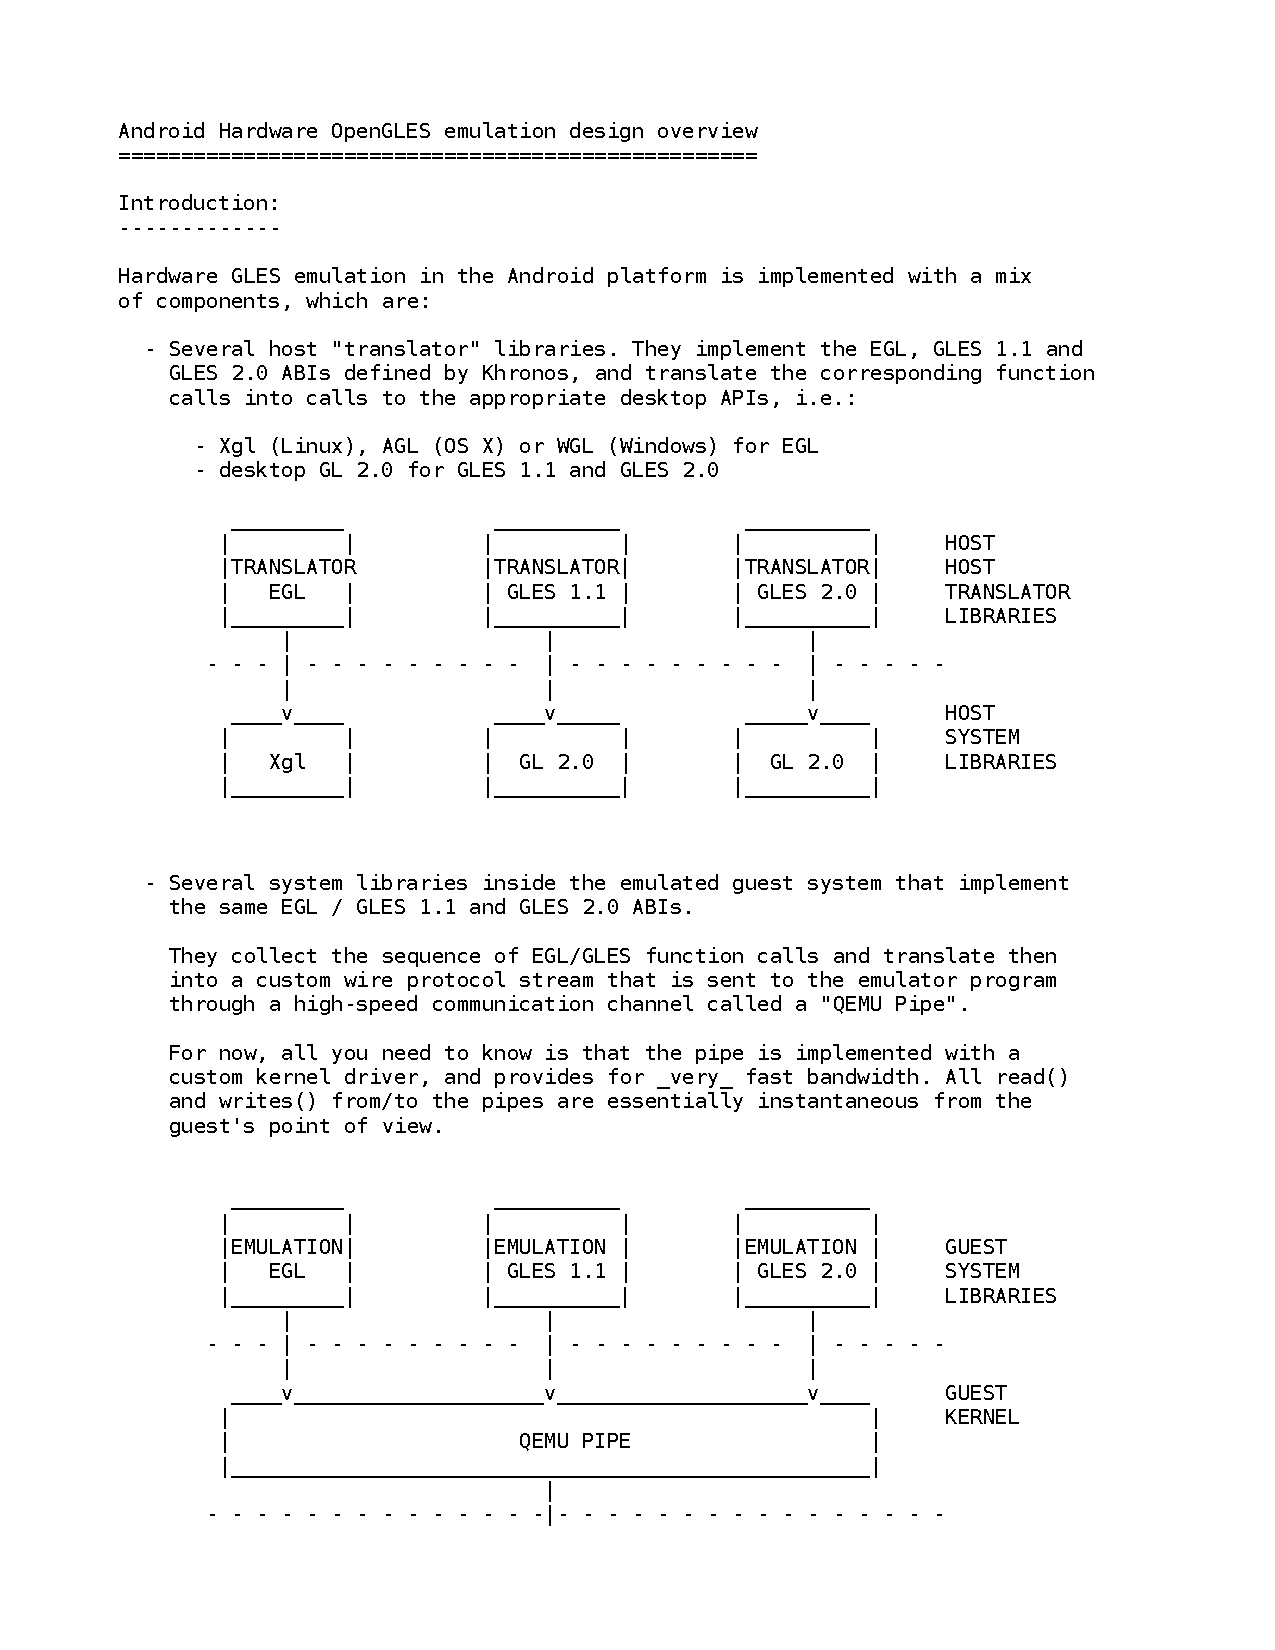
\includepdf[pages=-,scale=.8,pagecommand={}]{../dv2524-encl/androidopenglesdesignoverview.pdf}


% Chapter (+) - Back page(s)
\newcommand{\commitlink}{https://github.com/CaterHatterPillar/dv2524/commit/}
\expandafter\def\expandafter\commitlink\expandafter{\commitlink \gitAbbrevHash}

\renewcommand{\dateseparator}{-} % To print date in same format as gitinfo-package.

{\pagestyle{empty}
\changepage{5cm}{1cm}{-0.5cm}{-0.5cm}{}{-2cm}{}{}{}
\noindent%
\begin{tabular}{p{\textwidth}}
{\small This document was compiled in \buildconfig\ \today\ and last edited by \gitAuthorName\ \gitAuthorDate . This document is Version.\gitVtagn , and can be identified using revision- and commit hash \href{\commitlink}{\texttt{\gitAbbrevHash}}}. % \gitReferences\
\end{tabular}

\par\vspace {22cm} % HACK %\vfill

\noindent%
\begin{tabular}{p{0.5\textwidth}lcl}
Dept. Computer Science \& Engineering & Internet & : & \url{www.bth.se/didd}\\
Blekinge Institute of Technology & Phone	& : & +46 455 38 50 00 \\
SE--371 79 Karlskrona, Sweden & Fax & : & +46 455 38 50 57 \\
\end{tabular}
\clearpage
} % Back to \pagestyle{plain}


\end{document}
